\documentclass{article}

\usepackage[UTF8]{ctex}
\usepackage{amsmath,amssymb}
\usepackage{geometry}
\usepackage{graphicx}

\geometry{a4paper, margin=2.5cm}

\begin{document}

% ============================================================
\section*{PPO（Proximal Policy Optimization）}

\subsection*{先讲一个故事}

你是一名武术选手，每次上场（一次 rollout）结束后，教练（优势函数 $\hat{A}$）给你一份详细的复盘报告：「第 23 秒的侧踢应该更快」、「第 47 秒的防守太保守了」。报告\textbf{基于你当时的打法}（旧策略 $\pi_{\theta_{\text{old}}}$）写成。

你拿到报告，朝最优方向调整一遍。感觉还不够，再调整一遍……调了 $K=20$ 遍之后，你已经变成了一个截然不同的选手——可教练的建议还是当初那份，基于二十轮前的你写的。你越按报告调，动作越奇怪，最终反而一败涂地。

\textbf{核心矛盾}：
\begin{itemize}
  \item 数据是旧策略 $\pi_{\theta_\text{old}}$ 收集的；
  \item 每轮更新的目标是新策略 $\pi_\theta$；
  \item 更新越多，两者越远——数据越失效。
\end{itemize}

这就是无约束多轮策略更新的困境，也是 PPO 要解决的核心问题：

\[
\boxed{\text{如何在不浪费样本的前提下，安全地多次更新策略？}}
\]

\subsection*{数学形式化}

策略梯度定理给出参数梯度方向：

\[
\nabla_\theta J(\theta) = \mathbb{E}_{\pi_\theta}\!\left[\nabla_\theta \log \pi_\theta(a_t \mid s_t)\,\hat{A}_t\right]
\]

为了重复使用旧策略收集的数据，引入\textbf{重要性采样权重}（策略比值）：

\[
\boxed{r_t(\theta) = \frac{\pi_\theta(a_t \mid s_t)}{\pi_{\theta_\text{old}}(a_t \mid s_t)}}
\]

$r_t = 1$ 表示新旧策略在该步完全一致；$r_t \gg 1$ 或 $r_t \ll 1$ 表示策略已经严重偏离。

代入代理目标（Surrogate Objective）：

\[
L^{\text{CPI}}(\theta) = \hat{\mathbb{E}}_t\!\left[r_t(\theta)\,\hat{A}_t\right]
\]

\textbf{翻译成人话}：把每步的优势 $\hat{A}_t$ 乘以「新旧策略的比值」，多次优化这个代理目标就能多次复用同一批数据。\textbf{问题是}：$K$ 轮更新后 $r_t$ 可能偏离 $1$ 很远，代理目标变得不可信，梯度方向失效。

% ============================================================
\section*{无约束更新为什么会崩溃？}

\subsection*{重要性采样的有效范围}

重要性采样的隐含前提是两个分布「足够相近」。若 $\pi_\theta$ 与 $\pi_{\theta_\text{old}}$ 差距过大，估计方差爆炸：

\[
\operatorname{Var}\!\left[r_t(\theta)\,\hat{A}_t\right] \propto \mathbb{E}\!\left[r_t^2(\theta)\right] - 1
\]

当 $r_t$ 偏离 $1$（无论偏大还是偏小），梯度估计的方差急剧增大，更新方向变得不可靠。

\subsection*{$K$ 轮更新导致 $r$ 漂移}

以无 clip 的 PPO（$K=20$ 轮）为例，每轮更新后 $\theta$ 改变，$r_t(\theta)$ 随之漂移：

\begin{itemize}
  \item 第 1 轮：$r_t \approx 1$，梯度估计可信；
  \item 第 4 轮：$r_t$ 开始偏离，优势估计出现偏差；
  \item 第 8 轮：$r_t$ 严重偏离，优势估计彻底失效，梯度方向错误，训练崩溃。
\end{itemize}

\begin{figure}[htbp]
  \centering
  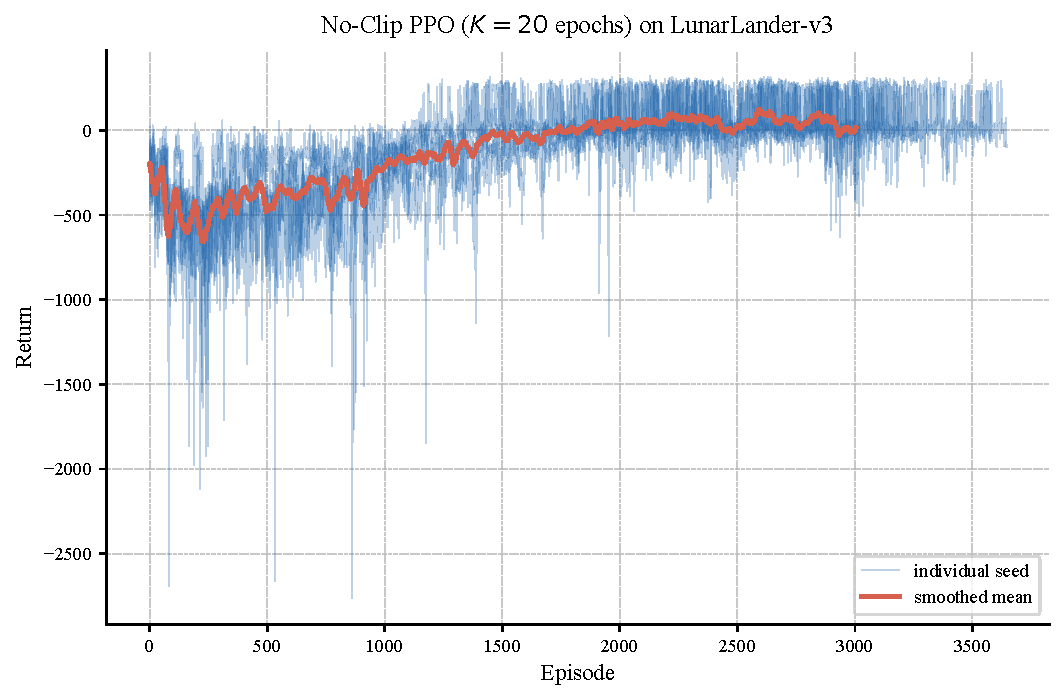
\includegraphics[width=\textwidth]{fig1_noclip_instability.pdf}
  \caption{无 clip 的 PPO（$K=20$ 轮，mini-batch）在 LunarLander-v3 上的 5 个 seed（蓝色细线）。
           部分 seed 在早期回报跌至 $-8000$（随机策略的 40 倍更差），随后缓慢恢复。
           平滑均值（红色）在整个训练期间始终低于有 clip 的版本。}
\end{figure}

% ============================================================
\section*{PPO-Clip：截断代理目标}

\subsection*{核心公式}

PPO 的解决方案极其简洁：\textbf{把 $r_t$ 截断到 $[1-\varepsilon,\;1+\varepsilon]$ 附近}，
超出部分不再提供梯度激励。

\[
\boxed{L^{\text{CLIP}}(\theta)
  = \hat{\mathbb{E}}_t\!\left[\min\!\left(
      r_t(\theta)\,\hat{A}_t,\;
      \operatorname{clip}\!\left(r_t(\theta),\,1-\varepsilon,\,1+\varepsilon\right)\hat{A}_t
    \right)\right]}
\]

$\varepsilon$ 通常取 $0.2$。

\subsection*{直觉：剪掉两种极端}

分两种情况理解 $\min$ 的含义。

\textbf{情况 A：$\hat{A}_t > 0$（这步动作比平均水平好，想增大它的概率）}
\begin{itemize}
  \item $r_t$ 增大（新策略更倾向此动作）$\to$ 好，但超过 $1+\varepsilon$ 时取 clip 值，梯度归零；
  \item \textbf{核心原则}：策略改动「已经够了」，不再继续推动。
\end{itemize}

\textbf{情况 B：$\hat{A}_t < 0$（这步动作比平均水平差，想减小它的概率）}
\begin{itemize}
  \item $r_t$ 减小（新策略远离此动作）$\to$ 好，但低于 $1-\varepsilon$ 时取 clip 值，梯度归零；
  \item \textbf{核心原则}：同上，过度回避也不再激励。
\end{itemize}

\underline{只有更新朝有利方向走且尚未超限时，才提供梯度驱动}。

\subsection*{clip 如何压制 $r$ 的漂移}

\begin{figure}[htbp]
  \centering
  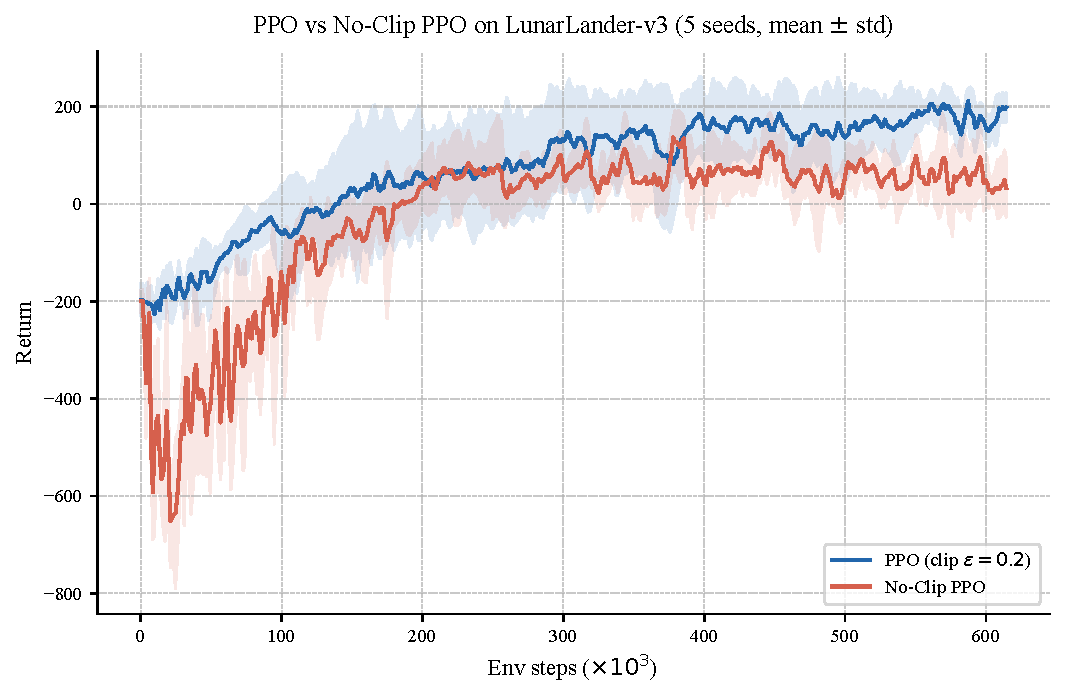
\includegraphics[width=\textwidth]{fig2_clip_vs_noclip.pdf}
  \caption{PPO-Clip（蓝）vs 无 Clip PPO（红）在 LunarLander-v3 上（5 seeds，均值 $\pm$ 标准差）。
           横轴为环境交互步数（$\times10^3$），两方法总步数完全相同（$300\times2048\approx614\text{k}$），
           排除了「好策略 episode 更长导致 episode 数更少」的混淆因素。
           Clip 版本稳定上升，约 400k 步后进入正回报区间；
           无 Clip 版本早期崩至 $-600\sim-1000$，缓慢恢复，始终落后且方差更大。}
\end{figure}

\begin{figure}[htbp]
  \centering
  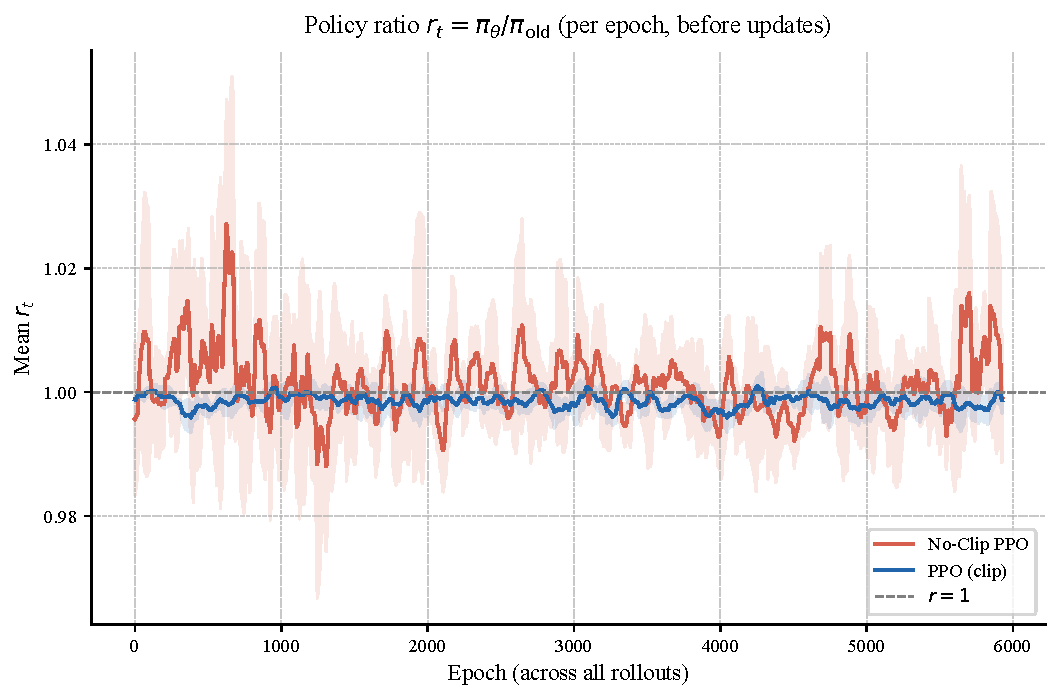
\includegraphics[width=\textwidth]{fig3_policy_ratio.pdf}
  \caption{每个 epoch 开始前、以全批数据测量的均值策略比值 $r_t$（5 seeds，均值 $\pm$ 标准差）。
           无 Clip（红）偏离更大，早期可达 $\sim\!1.017$；PPO-Clip（蓝）始终贴近 $1$。
           均值之外，个别 transition 的 $r_t$ 可远超 $1.2$ 的 clip 边界，正是这些尾部被 clip 截断，防止了错误梯度的累积。}
\end{figure}

\subsection*{为什么 clip 起作用？}

\begin{enumerate}
  \item \textbf{限制每步更新的「步幅」}：$r_t \in [1-\varepsilon, 1+\varepsilon]$ 等价于新旧策略的概率比不超过 $\pm 20\%$；
  \item \textbf{对称保护}：既防止某动作概率被过度增大，也防止被过度减小；
  \item \textbf{悲观下界}：$L^{\text{CLIP}}$ 是 $L^{\text{CPI}}$ 的下界，不会「自欺欺人」地高估提升量——只有真实提升时才更新。
\end{enumerate}

% ============================================================
\section*{广义优势估计（GAE）}

\subsection*{为什么需要 GAE？}

优势函数 $A(s,a) = Q(s,a) - V(s)$ 衡量「这步动作比平均水平好多少」。实践中有两种极端估计：

\[
\begin{array}{c|c|c}
\text{方法} & \text{偏差} & \text{方差} \\
\hline
\hat{A}^{\text{MC}} = \displaystyle\sum_{l=0}^{\infty}\gamma^l r_{t+l} - V(s_t) & \text{零偏差} & \text{极大} \\[6pt]
\hat{A}^{\text{TD}} = r_t + \gamma V(s_{t+1}) - V(s_t) & \text{有偏} & \text{极小} \\
\end{array}
\]

GAE 在两者之间插值，用 $\lambda \in [0,1]$ 控制偏差-方差权衡。

\subsection*{GAE 公式}

定义 TD 残差（一步时序差分误差）：
\[
\delta_t^V = r_t + \gamma V(s_{t+1}) - V(s_t)
\]

GAE 对指数加权的多步 TD 残差求和：

\[
\boxed{\hat{A}_t^{\text{GAE}(\gamma,\lambda)} = \sum_{l=0}^{\infty}(\gamma\lambda)^l\,\delta_{t+l}^V}
\]

等价的递推形式（实现中使用，从末尾向前归纳）：

\[
\hat{A}_t = \delta_t^V + \gamma\lambda\,\hat{A}_{t+1}
\]

\subsection*{$\lambda$ 的意义：在 TD 与 MC 之间插值}

\[
\begin{array}{c|c|c}
\lambda & \text{退化为} & \text{效果} \\
\hline
\lambda = 0 & \hat{A}_t = \delta_t^V \;\;(\text{1步 TD}) & \text{低方差，有偏差} \\[4pt]
\lambda = 1 & \hat{A}_t = \displaystyle\sum_{l=0}^{\infty}\gamma^l r_{t+l} - V(s_t)\;\;(\text{MC}) & \text{零偏差，高方差} \\[6pt]
\lambda = 0.95 & \text{实践中常用} & \text{偏差/方差折中} \\
\end{array}
\]

\textbf{翻译成人话}：$\lambda$ 越大，越相信实际采样的远期回报，而非 critic 的预测。PPO 通常取 $\gamma = 0.99,\;\lambda = 0.95$。

% ============================================================
\section*{PPO 完整算法}

\subsection*{总损失函数}

\[
\boxed{L^{\text{PPO}}(\theta)
  = L^{\text{CLIP}}(\theta)
  \;-\; c_1\,L^{\text{VF}}(\theta)
  \;+\; c_2\,S[\pi_\theta]}
\]

各项含义：
\begin{itemize}
  \item $L^{\text{CLIP}}$：截断策略梯度损失（最大化）；
  \item $L^{\text{VF}} = \hat{\mathbb{E}}_t\!\left[\left(V_\theta(s_t) - \hat{V}_t^{\,\text{target}}\right)^2\right]$：Critic 的均方误差（最小化，$c_1 \approx 0.5$）；
  \item $S[\pi_\theta] = \hat{\mathbb{E}}_t\!\left[-\sum_a \pi_\theta(a|s_t)\log\pi_\theta(a|s_t)\right]$：熵奖励，防止策略过早退化（最大化，$c_2 \approx 0.01$）。
\end{itemize}

Actor 和 Critic \textbf{共享网络参数} $\theta$，一次反向传播同时更新两者。

\subsection*{PPO-Clip 算法流程}

\begin{enumerate}
  \item \textbf{收集 rollout}：用 $\pi_{\theta_\text{old}}$ 在环境中运行 $T$ 步，记录 $(s_t, a_t, r_t, s_{t+1})$；
  \item \textbf{估计优势}：用 GAE 计算 $\hat{A}_t$，令回报目标 $\hat{V}_t^{\,\text{target}} = \hat{A}_t + V_{\theta_\text{old}}(s_t)$；
  \item \textbf{$K$ 轮 mini-batch 更新}：
    \begin{enumerate}
      \item 前向传播，计算 $r_t(\theta)$、$L^{\text{PPO}}(\theta)$；
      \item 梯度裁剪（$\|\nabla\theta\|_2 \le 0.5$），反向传播；
      \item 更新 $\theta$。
    \end{enumerate}
  \item 令 $\theta_\text{old} \leftarrow \theta$，返回第 1 步。
\end{enumerate}

\textbf{为什么 $K$ 轮更新安全了？} clip 把每步的 $r_t$ 限制在 $[1-\varepsilon, 1+\varepsilon]$，
即使 $K=20$，$\pi_\theta$ 也始终不会脱离 $\pi_{\theta_\text{old}}$ 的信任域。

% ============================================================
\section*{PPO vs 其他策略梯度方法}

\subsection*{一表打尽}

\[
\begin{array}{c|c|c|c}
\text{方法} & \text{样本效率} & \text{稳定性} & \text{实现复杂度} \\
\hline
\text{REINFORCE}  & \text{极低（每批更新一次）} & \text{低（高方差）}  & \text{最简单} \\
\text{A2C}        & \text{低（同上）}           & \text{中}            & \text{简单} \\
\text{TRPO}       & \text{高（$K$ 轮更新）}     & \text{高（KL 约束）} & \text{极复杂（二阶）} \\
\text{PPO-Clip}   & \text{高（$K$ 轮更新）}     & \text{高（clip 约束）} & \text{简单（一阶）} \\
\end{array}
\]

\subsection*{为什么 PPO 比 TRPO 更流行？}

TRPO（Trust Region Policy Optimization）用 KL 散度作硬约束：

\[
\max_\theta L^{\text{CPI}}(\theta)
\quad \text{s.t.} \quad
\hat{\mathbb{E}}_t\!\left[D_{\text{KL}}\!\left(\pi_{\theta_\text{old}}(\cdot\mid s_t)
  \;\|\; \pi_\theta(\cdot\mid s_t)\right)\right] \le \delta
\]

理论上最严格，但需要计算自然梯度（Fisher 信息矩阵求逆），在深度网络上成本极高。

PPO 把「信任域」变成\textbf{软约束}：超出部分不是被惩罚，而是\underline{不再提供梯度激励}。

\begin{itemize}
  \item \textbf{TRPO}：「越界了就罚」（硬约束，二阶优化）；
  \item \textbf{PPO}：「快到边了就不推了」（软约束，一阶优化）。
\end{itemize}

效果相当，但 PPO 仅需一阶梯度，实现简洁、速度快，成为在线策略方法的默认基线。

% ============================================================
\section*{本章在 RL 体系中的位置}

\begin{enumerate}
  \item \textbf{TD 路线} $\to$ Q-Learning $\to$ DQN（离散动作，值函数方法）；
  \item \textbf{MC 路线} $\to$ REINFORCE $\to$ 策略梯度（高方差，每批仅更新一次）；
  \item \textbf{Actor-Critic} $\to$ GAE $\to$ \underline{PPO}（本章：低方差 + 安全多轮更新）；
  \item \textbf{连续动作 / 离线场景} $\to$ SAC（最大熵 RL，离线友好）$\to$ 离线 RL（IQL 等）。
\end{enumerate}

PPO 是当前在线策略 RL 的默认基线——几乎所有 RLHF（大模型对齐）都以 PPO 为核心。
既然 PPO 已经如此稳健，为什么还需要为连续动作和离线场景单独设计新算法？

\subsection*{参考资料}

\begin{enumerate}
  \item Schulman et al.\ (2017). Proximal Policy Optimization Algorithms. \textit{arXiv:1707.06347}.
  \item Schulman et al.\ (2015). Trust Region Policy Optimization. \textit{ICML}.
  \item Schulman et al.\ (2016). High-Dimensional Continuous Control Using Generalized Advantage Estimation. \textit{ICLR}.
  \item Sutton \& Barto (2018). \textit{Reinforcement Learning: An Introduction} (2nd ed.). Chapter 13.
  \item 动手学强化学习（Hands-on-RL）. 第12章：PPO 算法.
\end{enumerate}

\end{document}
